\section{样例运行结果与测试}
\label{sec:experiments}

\subsection{样例城市线路信息}

\textsc{TravelAgency}系统使用的样例城市线路信息包含14个城市,540条线路。14个城市分别为:北京、青岛、银川、南京、上海、杭州、西安、武汉、长沙、广州、南宁、重庆、昆明、拉萨。包括了全国各大主要城市、大多数省会城市等等。

\begin{table}[h]
\centering
\begin{tabular}{cccc}
\toprule
航班班次 & 列车班次 & 客车班次 & 总计 \\
\midrule
10 & 30 & 500 & 540 \\
\bottomrule
\end{tabular}
\caption{线路班次数量}
\label{tab:line-info}
\end{table}

表 \ref{tab:line-info} 中给出了线路的基本信息。除了航班是根据城市重要程度人为指定以外,火车、客车的班次,是在事先划定了连通的城市之后,根据数量随机生成的。线路的时间是根据两地之间的距离以及线路类型生成的,而线路的出发时间都是在集合$\mathds H$中随机选择的。

\subsection{一个例子:从拉萨到杭州的旅行方案}

\begin{figure}[t]
	\centering
	\subfloat[最小风险策略方案]{
		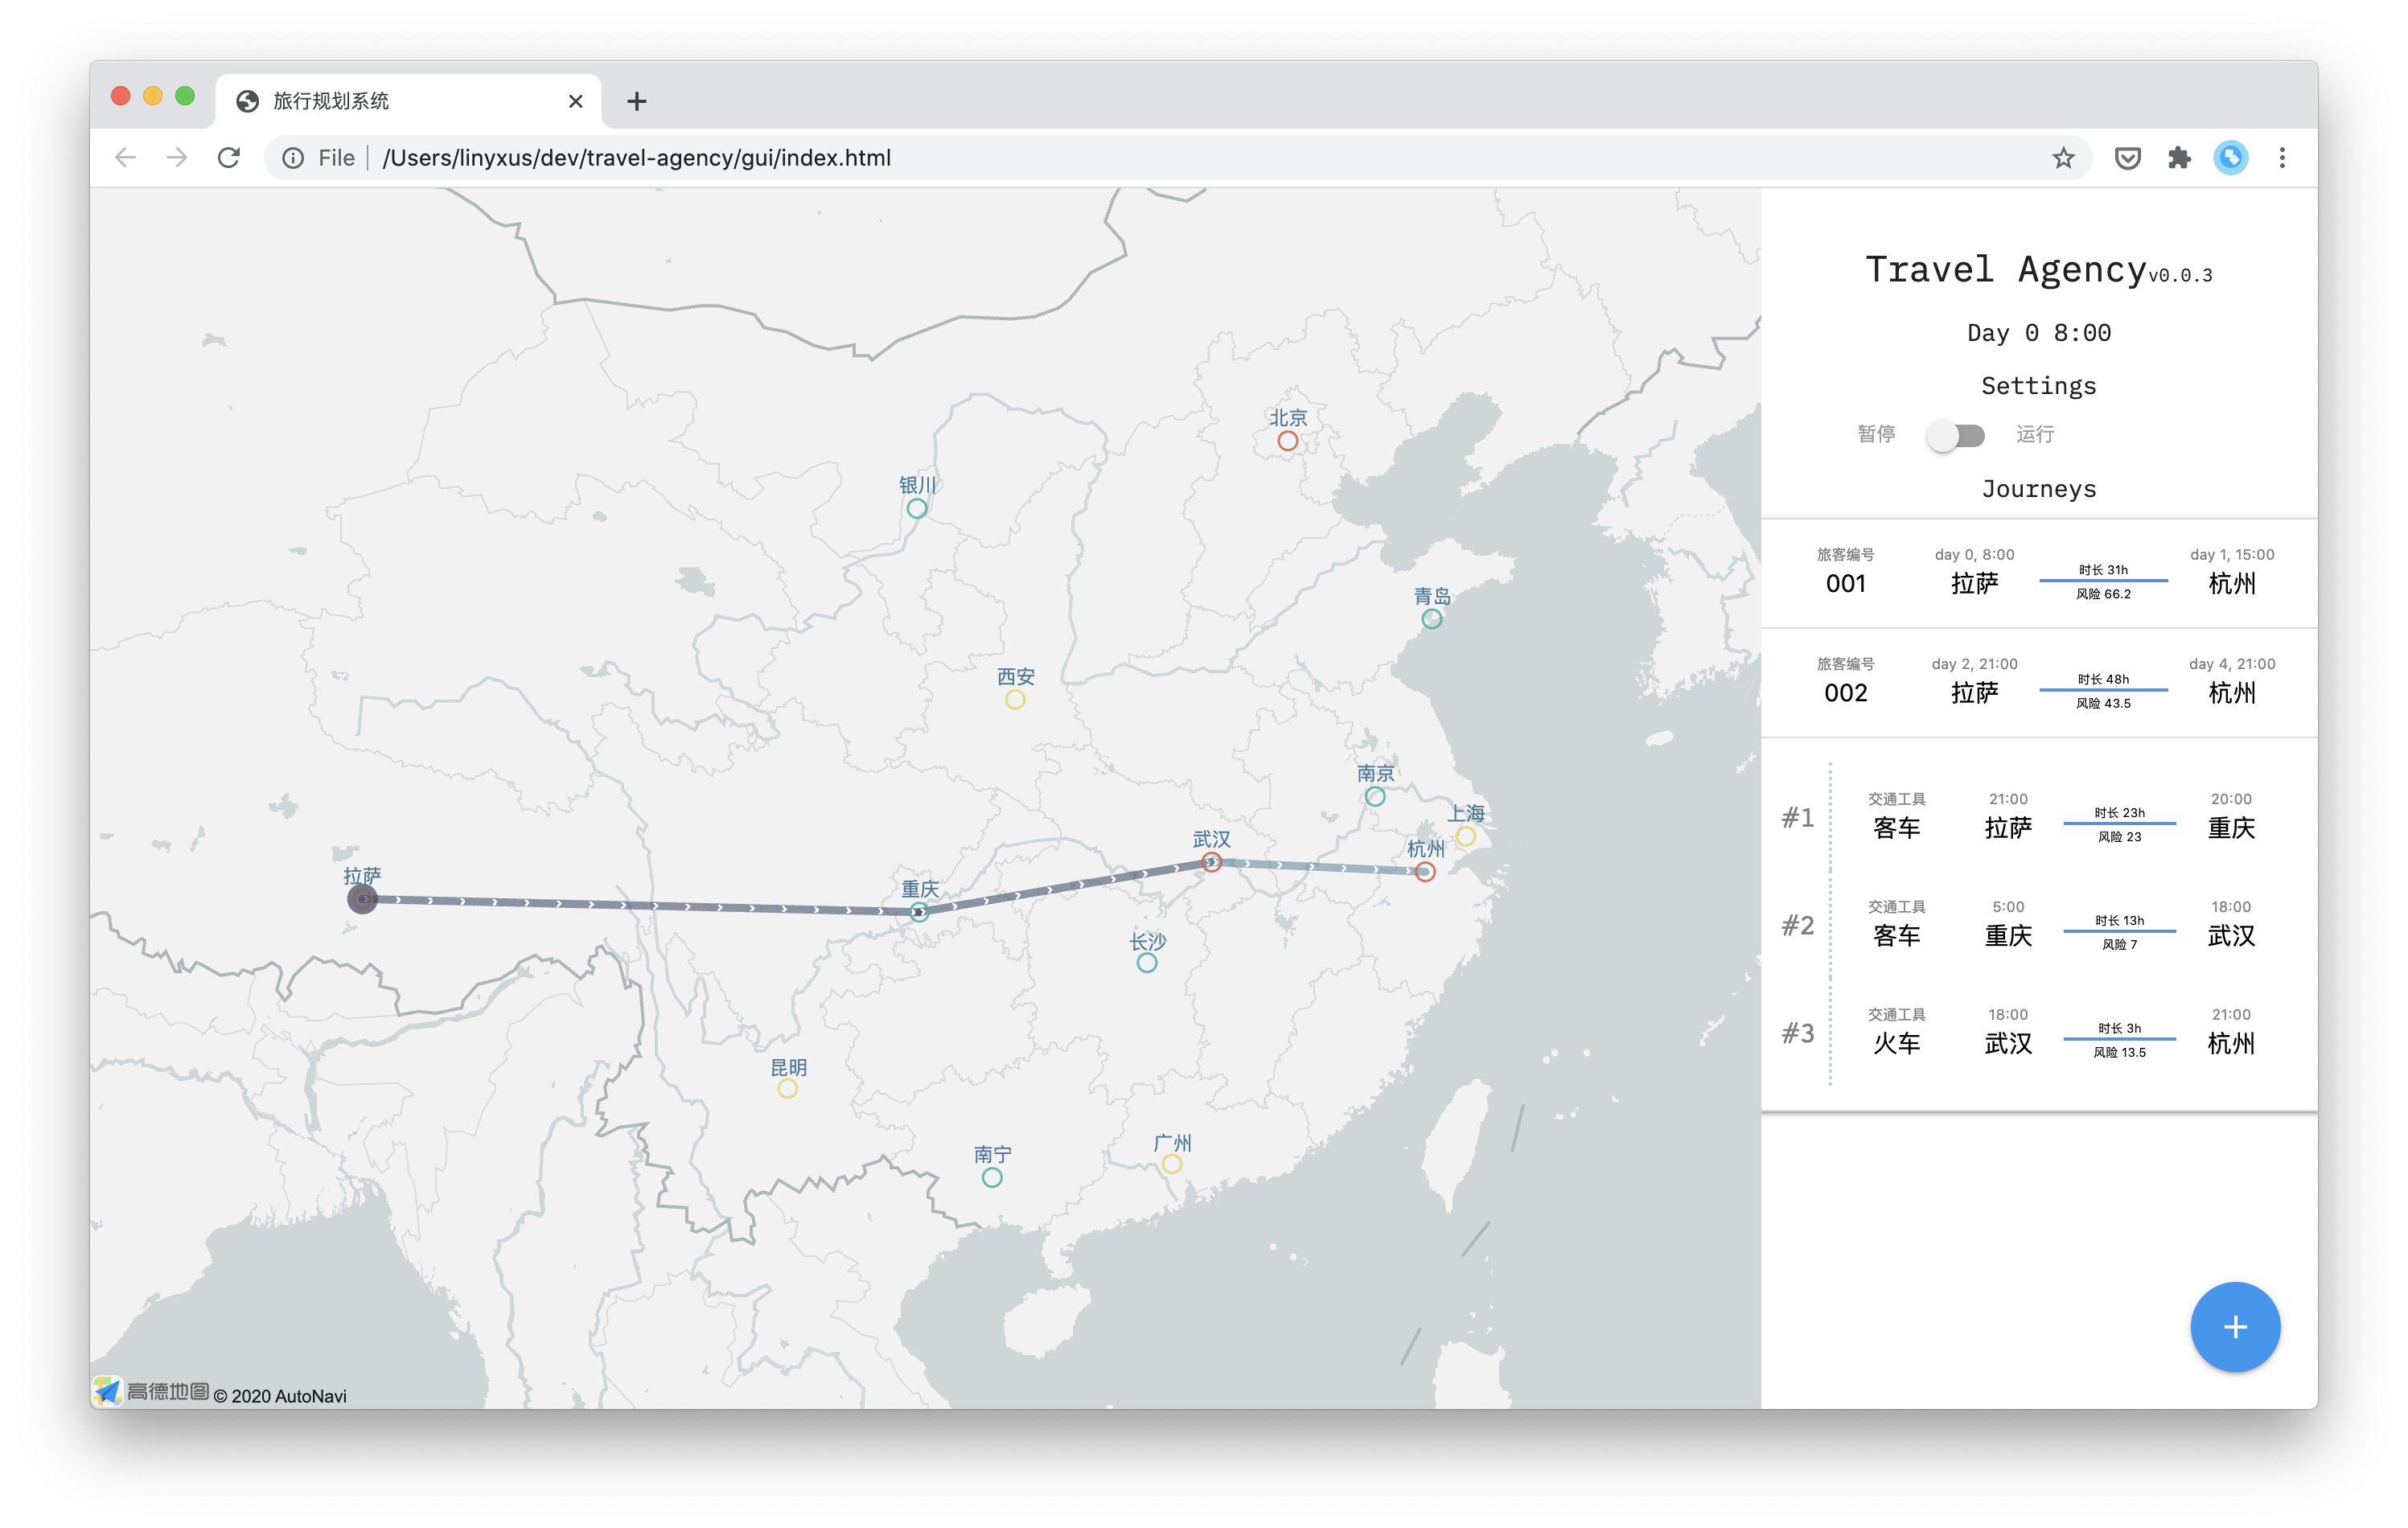
\includegraphics[width=0.5\textwidth]{figures/example_journey_mr}
		\label{fig:example-journey-mr}
	}
	\subfloat[限时最小风险策略方案]{
		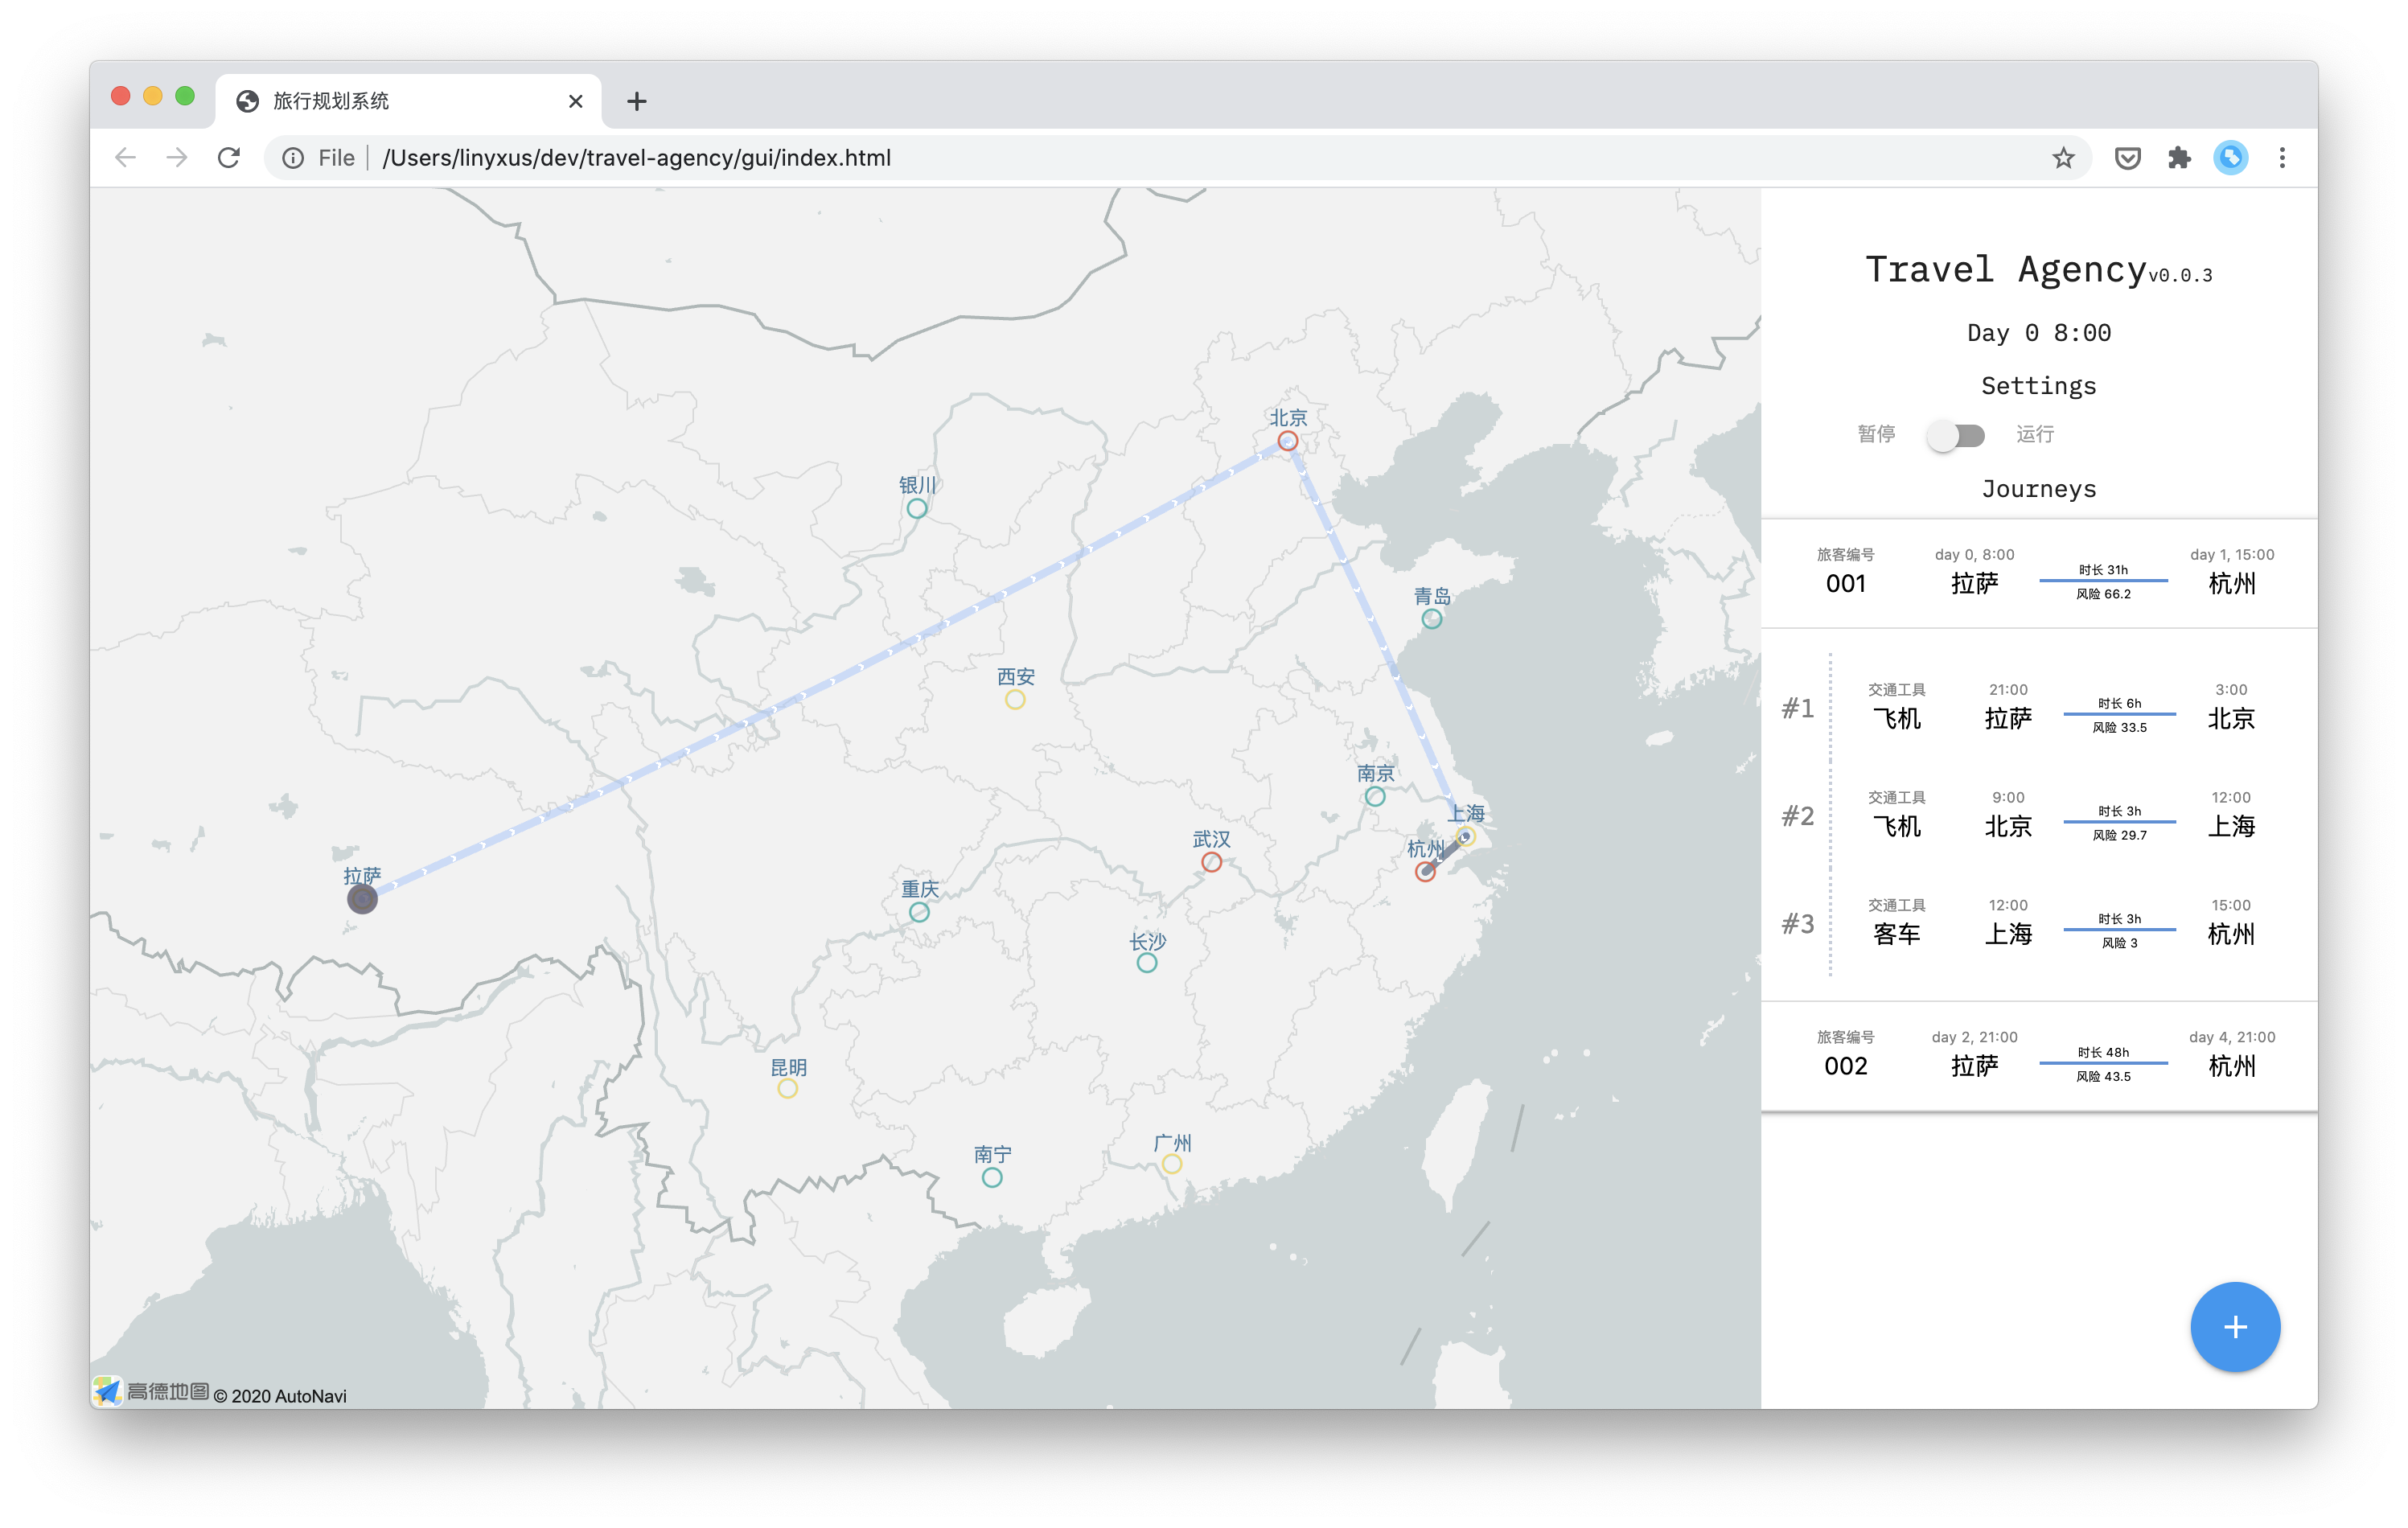
\includegraphics[width=0.5\linewidth]{figures/example_journey_ltmr}
		\label{fig:example-journey-ltmr}
	}
	\caption{从拉萨到杭州的旅行方案}
	\label{fig:example-journey}
\end{figure}

如图 \ref{fig:example-journey} 中所示,我给出了一个利用\textsc{TravelAgency}系统进行旅行规划的例子。例子中规划了从拉萨到杭州的旅行方案,图 \ref{fig:example-journey-mr} 中给出了最小风险策略的方案,图 \ref{fig:example-journey-ltmr} 中给出了限时40小时的最小风险方案。从图中可以看出,最小风险方案虽然风险最小,但是绕了远路,导致超出时间限制(需要48小时),而限时最小风险方案走了较为近的路程,且更多搭乘飞机,导致风险更大一些。

\subsection{单元测试}

在开发过程中,为C++编写的主要模块,借助GoogleTest测试框架编写了单元测试。主要有如下测试集:
\begin{enumerate}[(a)]
  \item \textbf{\lstinline{CityMap}模块。} 主要测试了城市线路信息能否正确读取、处理。
  \item \textbf{\lstinline{Journey}模块。} 主要测试了Journey类的关键方法,是否正确构造,是否能正确转化为线路列表,是否正确求出风险值等等。
  \item \textbf{\lstinline{LinkedList}模块。} 主要测试了链表类的关键方法。能否正确添加元素、求长度等等。
  \item \textbf{\lstinline{Solver}模块。} 测试了两种旅行规划模块能否给出正确的结果。
\end{enumerate}
共有5个测试集,22个测试点。测试了系统的核心功能,保证代码质量。为了运行测试,需要首先编译工程,随后在工程的根目录内运行 \texttt{./build/default/test\_main}。工程可以通过所有测试点。









